\section{Motivation and Challenges}
\label{sec:Motivation}

In domestic configurations, \IOT devices may be used in many different ways for many purposes. These devices are usually used in combination with each other in order to fulfil larger goals required by end users. Furthermore, for the same set of devices, say a temperature sensor and a connected heating system, the way they communicate (or not) can be very dissimilar. For example, in some situations the temperature sensor will regulate the heating system, where in other circumstances, it will be used to prevent fire situations. 

Considering the wide range of possible use cases for nowadays devices must be coupled to the profusion of vendors, hardware,\textsc{Api}s and so forth, which overburden the work of \IOT technicians when dealing with end user requirements. Besides the need for more standardization in \IOT specifications, there is also a crucial need for abstract definition of the semantics of \IOT configurations~\cite{park-16}. In order to illustrate our proposal, we will use an hypothetical \IOT configuration depicted in Figure~\ref{fig:scenario} where Alice's apartment is represented with a set of sensors and actuators.

\begin{figure}%
	\centering  
	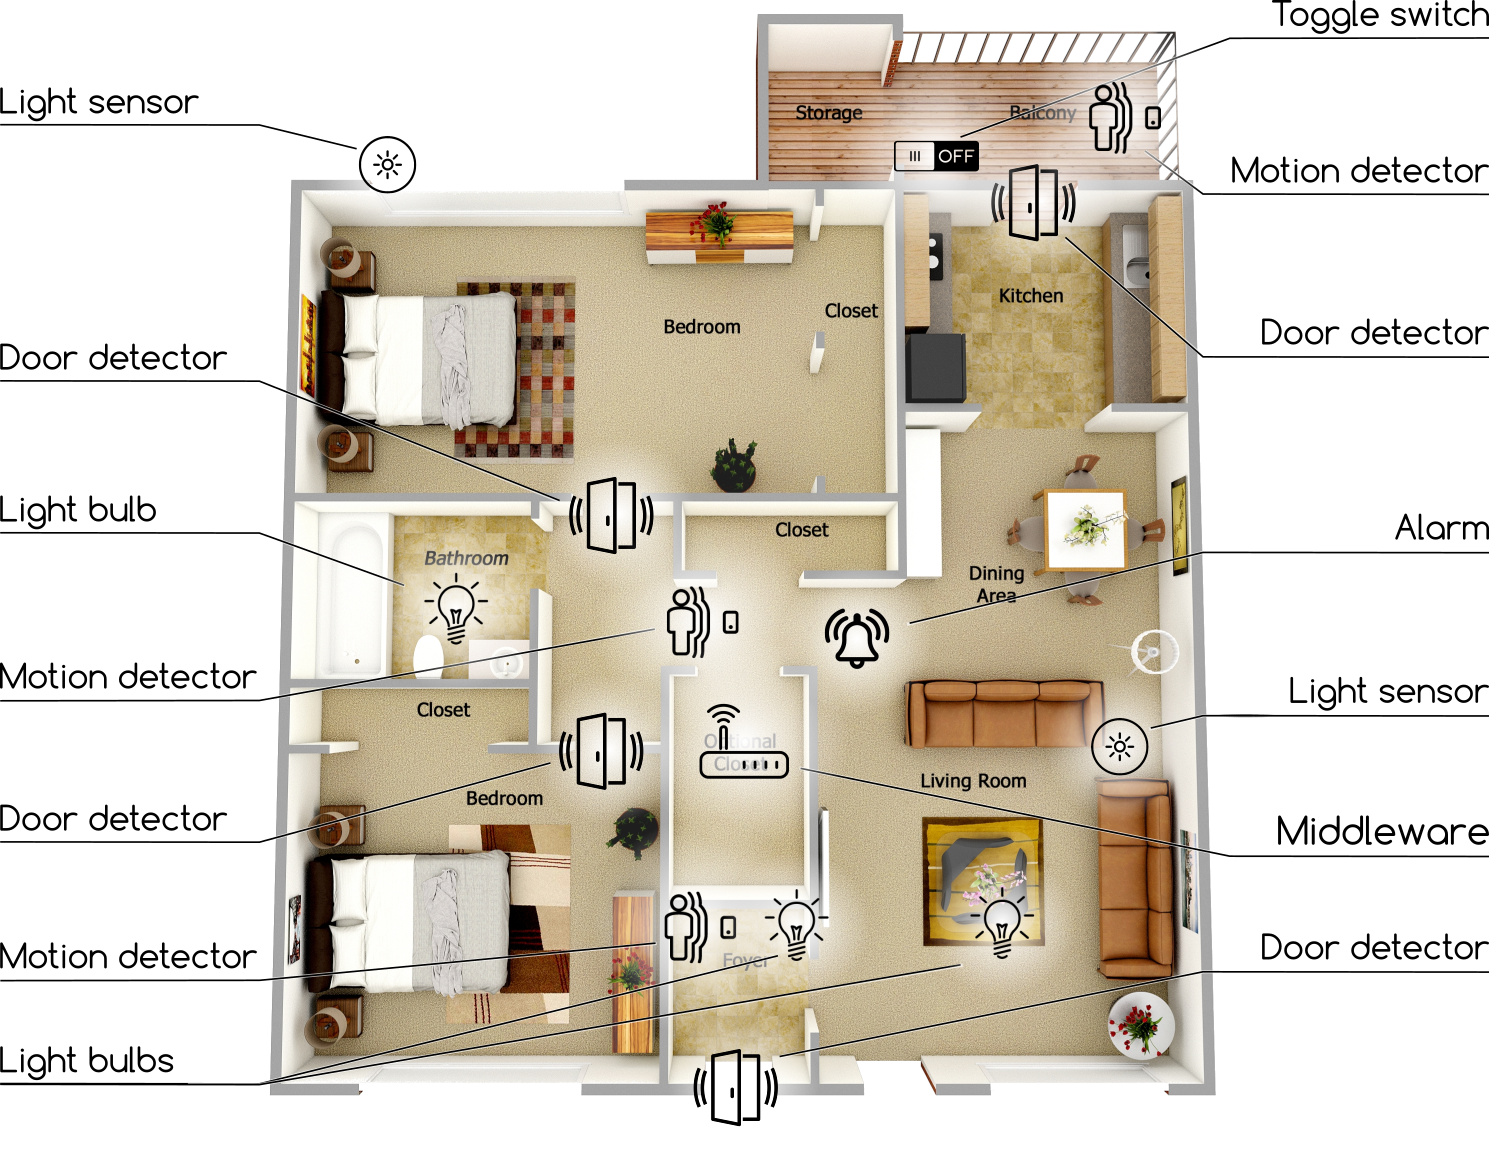
\includegraphics[width=.9\linewidth]{scenario.png}%
	\caption{Hypothetical Alice's \textit{smart-home} configuration of \IOT devices}%
	\label{fig:scenario}%
\end{figure}

This typical smart home configuration consists of light sensors and bulbs to handle the light in the apartment, motion and door detectors to verify the presence of persons, an alarm in case of emergency and a toggle switch on the balcony. Even if the amount of types of devices is rather limited, we can already highlight a set of features absolutely needed to describe the devices, network configuration and specify its dynamic aspects.

\begin{description}
	\item[Device Description] We need facility to make a precise inventory of the devices used in a specific deployment as well as the high-level capabilities of these devices, described in terms that are immediately understandable by end-users, as opposed to conveying technical details about how those devices precisely operate;
	
	\item[Network Description] A way to capture where each device is located and how it is possible to communicate with it, in order to receive or send data to it;
	
	\item[Dynamics] A way to describe the interactions wished by end-users, \textit{i.e.} how to leverage the functionalities of the devices to effectively realise one or several scenarios that are convenient for the end-users.  
\end{description}

Those three features are obviously not sufficient to obtain a fully-fledged solution that becomes adaptable to any situation, but they still represent necessary steps to provide end-users the capacity to manipulate a collection of devices without relying on specific technologies. Though, the definition of such \DSLS should encompass a series of facilities dedicated to hide the hardware-related constraints, but still user-defined abstract models should be somehow \textit{transformable} and \textit{traceable} into concrete infrastructures with simulation and verification possibilities. We particularly mention the following challenges:

\begin{description}
	\item[Capability Discovery] Providing the ability to drive interconnected devices assumes the capacity of automatically discovering devices' capabilities in a standardised and uniform way~\cite{chaqfeh-12}. Similar processes exist for other technologies, like \textsc{Usb} devices plugged into computers that automatically expose their natures and capabilities. Classifying those capabilities should be useful to build an ontology of normalised functions that could result in powerful \textsc{Api}s to manipulate devices. 
	
	\item[Reusability] Knowledge exchange and reusability of devices' definitions and interaction specifications are essential prerequisites to the adoption of a \DSL for the \IOT. It is not uncommon to reuse existing scenarios that involve a set of devices in different configurations. Those partial \IOT structures with their event orchestrations should be \textit{externalisable}, despite the large amount of standards, \textsc{API}s or hardware~\cite{ma-14}.

	\item[Complex Event Processing (\CEP)] Letting end-users deal with devices through their low-level capability interfaces could lead to confusion and stiff complexity for defining usage scenarios~\cite{ma-13}. Rather, providing a way of reifying low-level device computations into high-level events could help end-users leverage the complexity of devices networks and pave the way to manipulate them freely and transparently \cite{cugola-12}. Since \CEP consists of deriving meaningful conclusions from a stream of events occurring within a system and responding to them as quickly as possible, it provides a solution to extract meaningful events from low-level computations. However, for a solution to be complete and useful, the reverse operation should be addressed: high-level actions should be adequately translated into low-level actuations and interactions.
	
	\item[Protocol Interoperability] A smart-home solution with heterogeneous devices would often integrate elements from various providers, thus communicating through disparate protocols. In order to make them interact efficiently without forcing end-users to stick with one vendor, a powerful \DSL should provide ways for interoperability over multiple communication protocols, without requiring end-users to understand the protocols' intricacies, versions and technical restrictions~\cite{gubbi-13}.
	
	\item[Scalability] As the number of application domains increases, the amount of connected devices is expected to rise exponentially. When updating existing \IOT configurations, current solutions may not collapse when adding more elements~\cite{mukho-14}. Furthermore, a \DSL must provide a way to absorb scalability problems, hiding as much as possible purely technical constraints regarding increases in size and complexity of operating configurations. 
	
	\item[Data Management] Analogously to scalability issues, the massive increase in connected devices will produce more and more data to be processed, stored and, for some of them, post processed~\cite{lee-15}. More data means seemingly more storage capabilities and the required space to handle such flow of information will be at its highest ever. Furthermore, the multiplication of available (sensors) sources is creating a whole new world of data processing and mining possibilities, but also a profusion of divergent concrete data types that sooner or later must be mapped to equivalent concepts.
	
	\item[Non-Functional Properties] A powerful \DSL should encompass typical non-functional properties of device networks to ensure long-life and secure realisation of scenarios. \emph{Performance} is crucial, and depends both on the devices capabilities but also on the quality of the communication network. \emph{Resource availability}, both in terms of computation and memory capability, but also in terms of energy, is another crucial bottleneck for the adoption of \textsc{Dsl}s as a solution for defining scenarios. The generated code from the \DSL should not overload the devices with repetitive communications or unnecessary computations that would drain the device's battery. \emph{Security} is yet another concern with respect to two aspects. First, sensitive data could be exposed through the communication network, endangering users privacy. Second, some functionalities could be locked and only accessible to authorised users~\cite{tan-10}.
\end{description}